\section{Trees and storage layout}
\label{sec:layout}

\subsection{Counted, summarised copy-on-write trees}
\label{sec:tree}

Every tree in HStore is a B+tree over signed 64-bit keys. A leaf holds sorted keys and their values; a branch holds separator keys and child references. Nodes are never changed once another version can see them. An update copies the path from the root to the changed leaf, and the new root shares every other subtree with the old one, as in other copy-on-write B-trees~\cite{lorie,rodeh-shadowing,lmdb}. Inside one transaction, a node that the transaction itself created may be changed in place: each node carries an owner token, and a write copies a node only if its token is not the transaction's. A transaction that makes $n$ changes under one root therefore allocates in proportion to $n$ plus the nodes it touches, not $n$ times the tree height. When a version escapes, for example to a stream handed to the caller, the token is replaced and every node created so far becomes immutable.

Leaves are filled by bytes, not by entry count. A leaf tracks the exact size of its delta-encoded key stream and an upper bound on the size of its values, and splits when the total exceeds the page budget. With the default 16\,KiB page, a leaf of plain 8-byte keys holds thousands of entries and a branch holds up to 137 children.

\paragraph{Summaries.} Each child reference stores the subtree's \emph{summary}, a monoid value made of the entry count, the minimum and maximum key, the sum and range of the entry weights, the range of the validity intervals, a 64-bit mask of the role sets present, and a fingerprint. Combining two summaries is component-wise: sums, minima, maxima and bitwise or. The count makes rank, select and range counts logarithmic, since they subtract or add child counts from the references without loading the children. The other fields let a cursor skip any subtree that cannot hold a match: a scan for members valid at time $t$ enters a child only if $t$ lies in the child's time range, and a scan by role only if the role's bit is set in the mask. The mask is a 64-bucket Bloom filter, so a set bit only means ``maybe'' and the scan checks the role exactly.

\paragraph{Fingerprints.} Let $h(e)$ be a 64-bit hash of an entry. A tree whose order does not matter, such as the members of a set hyperedge, has the fingerprint $F(S)=\sum_{e\in S} h(e) \bmod 2^{64}$, an additive multiset hash~\cite{multiset-hash}. A sequence uses a polynomial hash~\cite{karp-rabin}, $F(e_1\ldots e_n)=\sum_i h(e_i)\,B^{\,n-i} \bmod 2^{64}$, whose concatenation rule $F(LR)=F(L)\,B^{|R|}+F(R)$ lets a branch combine its children's fingerprints. Both depend only on the contents, never on the shape of the tree or the order of insertion. Two hyperedges with different fingerprints differ, and the engine knows it after reading two references. All hashes are computed from explicit mixing functions, not from Java's object hash codes, so fingerprints stay the same across processes and across the native build.

\paragraph{Algebra on shared structure.} Because versions share subtrees, comparing two of them can skip whatever they share. Each reference to a stored subtree is identified by its page number, and two equal references denote the same subtree. A diff walks two frontiers of subtrees and drops a pair of equal references without reading it, so the diff of two consecutive generations costs about twice the tree height in page reads. Counting the intersection of two trees descends both in step: disjoint key ranges contribute nothing, equal references contribute their stored count, and only the parts that differ are read. Intersecting $k$ incidence sets uses a leapfrog join~\cite{leapfrog} over $k$ cursors, each restricted by summaries to the key range common to all inputs. A union of two trees with disjoint key ranges is a concatenation that copies $O(1+\Delta h)$ nodes, where $\Delta h$ is the difference in height.

\subsection{Hyperedges}
\label{sec:hyperedges}

The members of a set hyperedge are a tree keyed by member atom id, whose values are incidences. Membership tests and the member at rank $i$ are logarithmic, and the cardinality is the count in the root reference.

An ordered hyperedge is a sequence that can be edited at any position, so its keys are \emph{order-maintenance labels}~\cite{dietz-sleator,bender-order}: sparse integers in $[0,2^{62})$ whose order is the sequence order. The incidence stores the member id. An insertion between two members takes the midpoint of their labels; an append steps by $2^{24}$, so appending never relabels. When two neighbours have no free label between them, the engine relabels a window around the position, doubling its width until the free space reaches $2^8$ labels per member, which keeps the amortised cost of an insertion logarithmic. A second tree maps each member to its label, so membership tests stay logarithmic. Relabelling changes keys but not contents, so the fingerprint of an ordered hyperedge, which is computed from the incidences and not from their labels, does not change.

Incidence leaves are encoded column by column. A flag byte says which of the six optional columns (roles, weight, start and end of validity, payload, qualifier) any row in the leaf uses. Each such column has a bitmap of the rows that use it, followed by their values as variable-length integers. A plain membership therefore costs one to three bytes, and a leaf whose rows use no optional column is decoded into nothing but an array of member ids.

\begin{figure*}[t]
\centering
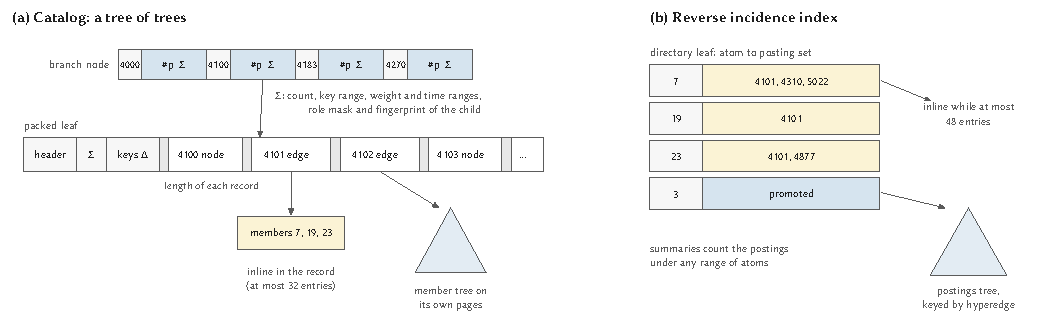
\includegraphics[width=\textwidth]{figures/layout}
\caption{(a) The catalog holds atom records. A hyperedge record holds its membership tree inline when the tree is one small leaf and points to its own pages otherwise. Every record in a catalog leaf is preceded by its length. (b) The reverse incidence index maps an atom to the hyperedges that contain it. Small posting sets are stored in the directory leaf, large ones in a tree of their own.}
\label{fig:layout}
\end{figure*}

\subsection{The catalog: a tree of trees}

The catalog maps an atom id to its record (\cref{fig:layout}a). A hyperedge's record holds references to the root of its membership tree and, for ordered hyperedges, of its label index. These are nested trees that the engine writes, counts and compacts like any other.

Most hyperedges are small: in the dataset of \cref{sec:evaluation}, the mean cardinality is 3.6. Giving each membership a page of its own would cost a page write, a cache entry and a page read for every hyperedge read. A nested tree is therefore kept \emph{inline} in its record when it is a single leaf of at most 32 entries whose encoding fits in 108 bytes, the space a record already reserves for a reference to a tree that is still in memory. That rule keeps pages from overflowing. While a hyperedge is being changed, the leaf that holds its record is sized as if the reference took the full 108 bytes. When the leaf is written, the reference becomes either a stored or an inline one, both of which fit in that space, so the written leaf can only shrink. The decision is made again each time the tree is written, so a hyperedge that grows past the limit moves to its own pages at the next checkpoint and one that shrinks moves back.

\subsection{The reverse incidence index}

The reverse index maps an atom to the hyperedges that contain it (\cref{fig:layout}b). It is a two-level structure. A directory tree maps the atom to a posting set; a posting set maps a hyperedge id to the member's roles and its position key in that hyperedge. A posting set is stored inline in the directory leaf while it has at most 48 entries and at most half the largest value size, and is promoted to a tree of its own beyond that. It is demoted again when it shrinks to 24 entries, so a set that hovers at the limit does not move back and forth. The directory's summaries add up posting counts as weights, so the number of incidences of any range of atoms is read from the summaries alone. The index is a derived slot: a derivation applies every membership change in a transaction to it before the transaction commits, so the two directions always agree within a generation.

\subsection{Node images, page numbers and segments}
\label{sec:pages}

A node is stored as an \emph{image}: an 80-byte header followed by the encoded node. The header holds a magic number, the page type, the tree's schema id, the node's own page number, the generation that wrote it, the payload length, the entry count, the node's summary and a CRC-32C over everything except the checksum itself. Every read verifies the magic number, the format, the page number and the checksum.

A page number is permanent. It has a 48-bit index and 16 bits reserved for reuse, and it says nothing about where the image is stored. The \emph{page directory} maps each index to an address made of a 24-bit segment number, a 24-bit offset in 64-byte units and a 16-bit length in units. The directory is a file of 8-byte entries, memory-mapped in 8\,MiB chunks, so a lookup is one load and takes no Java heap. Trees, the node cache and the log refer only to page numbers; only the page store resolves addresses. Page \code{\#1234}, stored in three units at unit 1234 of segment 1, is the directory entry at byte $64+8\cdot1234$, pointing to byte $64\cdot 1234$ of segment file \code{00000001.seg}.

Images are packed back to back into append-only segment files and aligned to 64 bytes, rather than given a fixed slot of the page size. A hypergraph produces many small nodes, and on the example database that ships with HStore packing cuts the segment space from 17.6\,MB to 1.0\,MB. Each segment is mapped read-only, and a read copies the image out of the map into a heap array before decoding it. Decoding straight from the map was two to five times slower in a microbenchmark, because the JIT compiler generates its fastest code only when every byte buffer that reaches the decoder is of the same kind, and the log and the catalog are decoded from heap arrays.

\subsection{Packed leaves and the node cache}
\label{sec:cache}

Decoded nodes are cached on the Java heap in a node cache with 16 shards. Each shard is an open-addressing table keyed by page number with a CLOCK ring~\cite{clock} for eviction and a byte budget. Lookups are lock-free; only admission takes the shard's lock. A node is charged an estimate of its heap size, computed from its arrays and entries with constants measured against the retained heap at two dataset sizes.

Catalog and index leaves hold variable-length records, and a fully decoded catalog leaf takes far more heap than its page. On our dataset a decoded catalog leaf of about 83 records, with their inline member lists, took about eleven times the size of its 1.5\,KiB image. With a cache smaller than the catalog, lookups missed the cache about half the time and each miss decoded every record of the page to return one. Leaves of codecs whose values are independent of each other therefore prefix every record with its length. A leaf read from a page is kept \emph{packed}: it holds the image, the decoded keys and the offset of every record, and decodes a record the first time it is read. The decoded record is published into the leaf with a compare-and-set, so concurrent readers see a whole record and keep whichever decoding finished first, and its estimated size is charged to the leaf's cache slot. A charge evicts other entries until the shard is back within its budget, and a charge for a slot that was evicted in the meantime is dropped. The length prefix costs about one byte per record; \cref{sec:eval-ablation} measures what it buys.
